%\documentclass{beamer}
\documentclass[aspectratio=169]{beamer}
\usetheme{Boadilla}
%\usetheme{Warsaw}
%\setbeamercovered{transparent}
\beamertemplatetransparentcoveredhigh
\usepackage[portuges]{babel}
\usepackage[utf8]{inputenc}
\usepackage{lmodern}
\usepackage[T1]{fontenc}
\usepackage{hyperref} 
\usepackage{listings}
\usepackage{color}

\definecolor{dkgreen}{rgb}{0,0.6,0}
\definecolor{gray}{rgb}{0.5,0.5,0.5}
\definecolor{mauve}{rgb}{0.58,0,0.82}

\lstset{frame=tb,
  language=C,
  aboveskip=3mm,
  belowskip=3mm,
  showstringspaces=false,
  columns=flexible,
  basicstyle={\small\ttfamily},
  numbers=none,
  numberstyle=\tiny\color{gray},
  keywordstyle=\color{blue},
  commentstyle=\color{dkgreen},
  stringstyle=\color{mauve},
  breaklines=true,
  breakatwhitespace=true,
  tabsize=3
}
\title[Cadeia de caracteres: Strings]{Cadeia de caracteres: Strings\\
   Algoritmos e Estrutura de Dados I}
\author[IEng - UFMT]{Instituto de Engenharia -- UFMT}
%\institute[2020/2]{Segundo Semestre de 2020}
\date{}


\begin{document}

%------------------------------------------------
\begin{frame}[plain]
  \titlepage
\end{frame}

%------------------------------------------------

\begin{frame}
\frametitle{Roteiro} % Table of contents slide, comment this block out to remove it
\tableofcontents % Throughout your presentation, if you choose to use \section{} and \subsection{} commands, these will automatically be printed on this slide as an overview of your presentation
\end{frame}

%----------------------------------------------------------------------------------------
%	PRESENTATION SLIDES
%----------------------------------------------------------------------------------------

%------------------------------------------------
\section{Objetivos}

\begin{frame}
\frametitle{Objetivos}
Esta aula tem como objetivos:

\begin{enumerate}
\item Apresentar os conceitos básicos sobre cadeias de caracteres;
\item Explicitar os exemplos de funções que manipulam cadeias de caracteres;
\item Exemplificar a execução desses algoritmos.
\end{enumerate}
\end{frame}


%------------------------------------------------
\section{Introdução} % Sections can be created in order to organize your presentation into discrete blocks, all sections and subsections are automatically printed in the table of contents as an overview of the talk
%------------------------------------------------

\begin{frame}
\frametitle{Introdução}
\begin{itemize}
\item Um caracter é considerado um tipo de dado primitivo.
\item Um tipo de dado é primitivo se o computador possui instruções em linguagem de máquina que permite a manipulação deste tipo.
\item Desde que uma cadeia é uma sequência de caracteres, o caracter é a entidade fundamental de manipulação de uma cadeia.
\end{itemize}
\end{frame}

\begin{frame}
\frametitle{Introdução}
\begin{itemize}
\item Um caracter pertence a um conjunto finito de caracteres: um alfabeto.
\item Um exemplo de alfabeto é o conjunto de letras da língua portuguesa.
\item Outro alfabeto comum é o conjunto de dígitos decimais.
\item Ao longo dos anos, vários alfabetos foram desenvolvidos para serem utilizados em computadores.
\end{itemize}
\end{frame}

\begin{frame}
\frametitle{Introdução}
\begin{itemize}
\item Caracteres literais são representados por aspas simples, como em 'A' ou 'a'.
\item Variáveis do tipo char podem receber valores literais do tipo caracter ou também valores inteiros (que nesse caso representam o caracter correspondente, conforme o sistema de condificação adotado)
\item Variáveis do tipo char podem também ter o seu valor comparado com inteiros.
\end{itemize}
\end{frame}

%------------------------------------------------

\begin{frame}
\frametitle{Introdução}
\begin{itemize}
\item Entre os vários métodos de codificação, os mais populares são:
  \begin{itemize}
    \item Código ASCII (7 bits) - American Standard Code for Information Interchange.
    \item Código EBCDIC (8 bits) - Extended Binary Coded Decimal Interchange Code.
    \item Código UNICODE (8 bits).
    \item Código UTF-8, nos dias de hoje substitui o sistema ASCII.
  \end{itemize}
\end{itemize}
\end{frame}

%------------------------------------------------

\begin{frame}
\frametitle{Tabela ASCII}
 
\begin{figure}[!h]
  \centering
  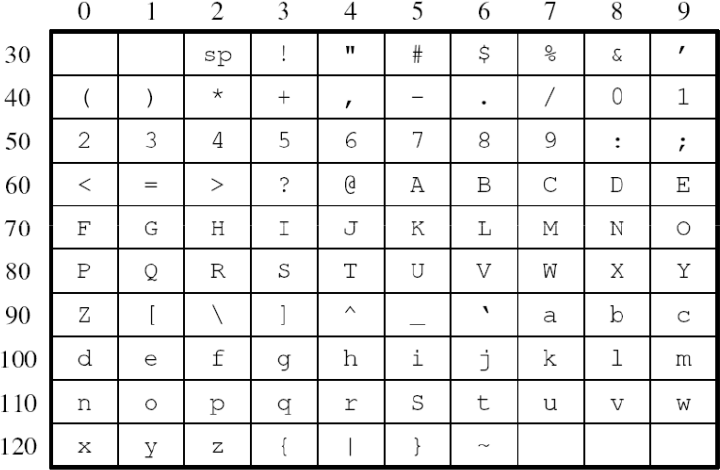
\includegraphics[width=300pt]{imgs/tabela_ascii.png}
  \label{fig_tabela_ascii}
\end{figure}
\end{frame}

%------------------------------------------------
\section{Cadeia de caracteres (strings)}

\begin{frame}
\frametitle{Cadeia de caracteres}
\begin{itemize}
\item Cadeia de caracteres (string): são sequências de letras, números ou símbolos onde o último caracter é o caracter nulo ( \textbackslash 0).
\item Na linguagem C utilizamos vetores do tipo char para armazenar cadeia de caracteres (strings).
\item Obrigatoriamente o último caracter é o caracter nulo. 
\item O caracter nulo serve para manipular a string sem correr o risco de acessar outras áreas de memória.
\end{itemize}
\end{frame}

%------------------------------------------------

\begin{frame}[fragile]
\frametitle{Cadeia de caracteres}
\begin{itemize}
\item Por exemplo, para declarar um espaço de memória que contenha 20 caracteres, fazemos:
    \begin{lstlisting}
    char nome[20];
    \end{lstlisting}
\item Inicializamos o vetor de caracteres da seguinte forma:
    \begin{lstlisting}
    char nome[20] = {'J','o','a','o','\0'};
    char nome[20] = "Joao";
    char nome[] = "Joao";
    \end{lstlisting}
\item Dessa forma, teremos:

\begin{figure}[!h]
  \centering
  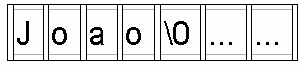
\includegraphics[width=75pt]{imgs/inicializacao.png}
  \label{fig_inicializacao}
\end{figure}
\end{itemize}
\end{frame}


%------------------------------------------------

\begin{frame}[fragile]
\frametitle{Cadeia de caracteres}
\begin{itemize}
\item Ao utilizar a função scanf() utilizando cadeia de caracteres, utiliza-se o código ``\%s''para leitura, omitindo o \&, que é utilizado em outros tipos. Por exemplo:
    \begin{lstlisting}
    printf("Digite o seu nome: ");
    scanf("%s", nome);
    printf("Seu nome eh %s.",nome);
    \end{lstlisting}

\end{itemize}
\end{frame}

%------------------------------------------------

\section{Exemplos}

\begin{frame}[fragile]
\frametitle{Exemplo}
Escreva um programa que leia uma palavra da entrada e imprima o número de caracteres desta palavra.
\end{frame}

%------------------------------------------------

\begin{frame}[fragile]
\frametitle{Cadeia de caracteres}
\begin{lstlisting}
#include<stdio.h>
int main() {
  char vetor[100];
  int i, n;
  printf("Digite uma palavra:");
  scanf("%s",vetor);
  i=0;
  while (vetor[i]!='\0') {
    i++;
  }
  printf("A quantidade de caracteres eh %d", i);
  return 0;
}
\end{lstlisting}

\end{frame}

\begin{frame}[fragile]
\frametitle{Exemplo}
Faça uma função que receba uma string e um caracter e verifica se o caracter esta contido na string. Caso o caracter seja encontrado, a funcao retorna a posicao em que o caracter se encontra na string. Caso contrario, retorna -1.
\end{frame}

%------------------------------------------------

\begin{frame}[fragile]
\frametitle{Cadeia de caracteres}
\begin{lstlisting}
int buscaCaracter(char string1[], char caracter) {
  int i = 0;
  while (string1[i]!='\0' && string1[i]!=caracter) {
      i++;
  }
  // Verifica se o contador i chegou no fim da string
  if (i==tamanhoString(string1)) {
    return -1;
  }
  // Retorna posicao da string
  return i;
}
\end{lstlisting}
\end{frame}
%------------------------------------------------

\begin{frame}[fragile]
\frametitle{Exemplo}
Faça uma função que receba uma string imprima cada caracter dessa string separado por um hífen.
\end{frame}


%------------------------------------------------

\begin{frame}[fragile]
\frametitle{Cadeia de caracteres}
\begin{lstlisting}
void imprimeString(char string[]) {
  int i = 0;
  while (string[i]!='\0') {
    printf("%c",string[i]);
    if (string[i+1]!='\0')
      printf("-");
    i++;
  }
  printf("\n");
}
\end{lstlisting}
\end{frame}

%------------------------------------------------

\begin{frame}[fragile]
\frametitle{Exemplo}
Faça uma função que receba duas strings e troque a primeira letra da primeira string com a última letra da segunda string.
\end{frame}

%------------------------------------------------

\begin{frame}[fragile]
\frametitle{Cadeia de caracteres}
\begin{lstlisting}
void trocaCaracteres(char string1[], char string2[]) {
  int i = 0, aux = 0;
  // Calcula o tamanho da segunda string
  while (string2[i]!='\0')
    i++;
  aux = string1[0];
  string1[0] = string2[i-1];
  string2[i-1] = aux;
}
\end{lstlisting}
\end{frame}

\begin{frame}
\Huge{\centerline{Dúvidas}}

\end{frame}

%----------------------------------------------------------------------------------------


\begin{frame}
  \frametitle{Fim}
\begin{center}
\Huge Fim
\end{center}
\end{frame}



\end{document} 